%\documentclass[aps,showpacs,prl,twocolumn,superscriptaddress]{revtex4}
\documentclass[%
%reprint,
superscriptaddress,
%groupedaddress,
%unsortedaddress,
%runinaddress,
%frontmatterverbose, 
preprint,
showpacs,
%preprintnumbers,
%nofootinbib,
%nobibnotes,
%bibnotes,
amsmath,
amssymb,
aps,
%pra,
prl,
%rmp,
%prstab,
%prstper,
%floatfix,
%twocolumn
]{revtex4-1}
\usepackage{amsmath}
\usepackage{graphicx}
\usepackage{booktabs}
\usepackage{multirow}
\usepackage{ulem}
\usepackage{color}
\usepackage{lipsum}
\usepackage[caption=false]{subfig}
\setcounter{footnote}{0}
%\usepackage[style=base]{caption}

\usepackage{array}
\newcolumntype{L}[1]{>{\raggedright\let\newline\\\arraybackslash\hspace{0pt}}m{#1}}
\newcolumntype{C}[1]{>{\centering\let\newline\\\arraybackslash\hspace{0pt}}m{#1}}
\newcolumntype{R}[1]{>{\raggedleft\let\newline\\\arraybackslash\hspace{0pt}}m{#1}}

\graphicspath{ {./Figures/} }

\begin{document}
	
\title{Exchange Magnons in Ferromagnetic Films Excited by Picosecond Acoustic Pulses}
	
\author{V. Besse}
\email{valentin.besse@univ-lemans.fr}
\affiliation{IMMM CNRS 6283, Le Mans Universit\'{e}, 72085 Le Mans cedex, France}
\author{A.V. Golov}
\affiliation{Syktyvkar State University named after Pitirim Sorokin, 167001, Syktyvkar, Russian Federation}
\author{V.S. Vlasov}
\affiliation{Syktyvkar State University named after Pitirim Sorokin, 167001, Syktyvkar, Russian Federation}
\author{A. Alekhin}
\affiliation{IMMM CNRS 6283, Le Mans Universit\'{e}, 72085 Le Mans cedex, France}
\author{D. Kuzmin}
\affiliation{Chelyabinsk State University, 454001 Chelyabinsk, Russian Federation}
\affiliation{South Ural State University (National Research University),454080 Chelyabinsk, Russian Federation}
\author{I.V. Bychkov}
\affiliation{Chelyabinsk State University, 454001 Chelyabinsk, Russian Federation}
\affiliation{South Ural State University (National Research University),454080 Chelyabinsk, Russian Federation}
\author{L.N. Kotov}
\affiliation{Syktyvkar State University named after Pitirim Sorokin, 167001, Syktyvkar, Russian Federation}
\author{V.V. Temnov}
\affiliation{IMMM CNRS 6283, Le Mans Universit\'{e}, 72085 Le Mans cedex, France}
	
\begin{abstract}
We present a numerical study of exchange magnons in nickel thin films excited by a series of picosecond acoustic pulses.
We use the Landau-Lifschitz-Gilbert equation to describe the magnetization dynamics and we consider the demagnetization energy, the external magnetic energy, the exchange energy and the magnetoelastic energy to describe the effective magnetic field.
The propagation of the strain due to the ultrashort acoustic pulses plays either on the magnetoelastic anisotropy or the exchange field and induced the magnetization dynamic.
We study the impact of the acoustic pulses characteristic on the propagating spinwave and the subsequent magnon orders.
We demonstrate the possibility to enhance certain modes by playing on the duration between two consecutive acoustic pulses in order to match the frequencies at which magnon and acoustic dispersion curves are crossing.
It is possible to tune the magnon dispersion curve by changing the magnitude of the external magnetic field or the angle between it and the out-of-plane direction.
\end{abstract}
	
\maketitle
	
The discovery ultrafast demagnetization by femtosecondes laser pulses in 1996 \cite{beaurepaire1996ultrafast} open the new and booming field of ultrafast
laser manipulation of magnetization \cite{koopmans2000ultrafast,van2002all,guidoni2002magneto,zhang2002coherent,vomir2005real,bigot2005ultrafast,kimel2005ultrafast,malinowski2008control,bigot2009coherent,bovensiepen2009femtomagnetism,radu2009laser,carpene2010ultrafast,boeglin2010distinguishing,radu2011transient,rudolf2012ultrafast,bombeck2013magnetization,kim2012ultrafast,kim2015controlling,kim2017magnetization}.
This control of magnetization precession is a key for further development in spintronic.
%The idea of data transmission by using the spins rather than electric currents had a large impact.
Magnetization dynamics induced by a pump laser pulse could be sort in different categories \cite{kirilyuk2010ultrafast}: thermal effects (laser-induced heating \cite{van2002all,carpene2010ultrafast}), photomagnetic effects (magnetocrystalline anisotropy) and optomagnetic effect (spin-orbit coupling, spin-transfer torque\cite{nvemec2012experimental,razdolski2017nanoscale,alekhin2017femtosecond}).
Nevertheless, the magnetic system of ordered substances is coupled with other systems as the elastic system, so the magnetization dynamics can also be driven by magnetoelastic effect \cite{beaurepaire1996ultrafast,kim2012ultrafast,bombeck2012excitation,temnov2012ultrafast,bombeck2013magnetization,kim2015controlling,januvsonis2016ultrafast,kim2017magnetization,chang2017parametric}.
In the case of a single ferromagnetic, we can limit our consideration just to two mechanisms: laser-induced heating and phonon-magnon interaction.

Previous work about magnetoacoustics dynamics demonstrated the possibility to controlled the precession by a series of picosecond acoustic pulses \cite{kim2012ultrafast,kim2015controlling,kim2017magnetization}.
They restricted the free energy $E$ to three contributions: the magnetocrystalline and magnetoelastic anisotropies, the demagnetization energy and the external magnetic field energy.
The propagation of the acoustic pulses induced a time dependent strain leading to a lattice deformation. %which generated the magnetization precession.
It modifies the magnetoelastic energy and drives the magnetization precession.
Using a method analogous to the Smit-Suhl method \cite{smit1955ferromagnetic,suhl1955ferromagnetic}, the authors describe the magnetization dynamics using the Landau-Lifschitz equation in spherical coordinates. 
Also they represented the acoustic pulse's excitation by either a Crenel function or a delta function assuming an instantaneous change in the magnetoelastic anisotropy.

Here, we report a numerical study of exchange magnons in nickel thin film excited by a series of picosecond acoustic pulses.
We show that the propagation of acoustic pulses through the film induces the generation and the propagation of a spinwave packet form by the magnon modes excited.
%The influence of the acoustic pulses' characteristics as the shape, the duration, the delay between the successive pulses and their number, is investigated.
%We present different matching condition between the acoustic and the magnon dispersion curve.
Fig.~\ref{fig:schemeGeometry} presents a scheme of the situation considered.
A DC magnetic field is applied to the film with an angle $\xi$ in relation to the film's plane.
It leads to a title of the equilibrium direction $\mathbf{m}_0$ of the magnetization vector.
Acoustic pulses propagate through the film and alter the direction of the effective magnetic field $\mathbf{H}_{\mathrm{eff}}$ thereby driving precessional motion of the magnetization.
Fig.~\ref{fig:schemeMovement} shows the resulting magnetization dynamic.
It can be decompose in two different motions: a precession P that describes the ferromagnetic resonance (FMR) and a nutation N which corresponds to the sum of the magnon modes.
%The effect on the induced magnetization dynamics induced is measured by monitoring the Kerr rotation angle at opposite side of ferromagnetic film.
\begin{figure}[ht]
	\centering
	\subfloat[]{\label{fig:schemeGeometry}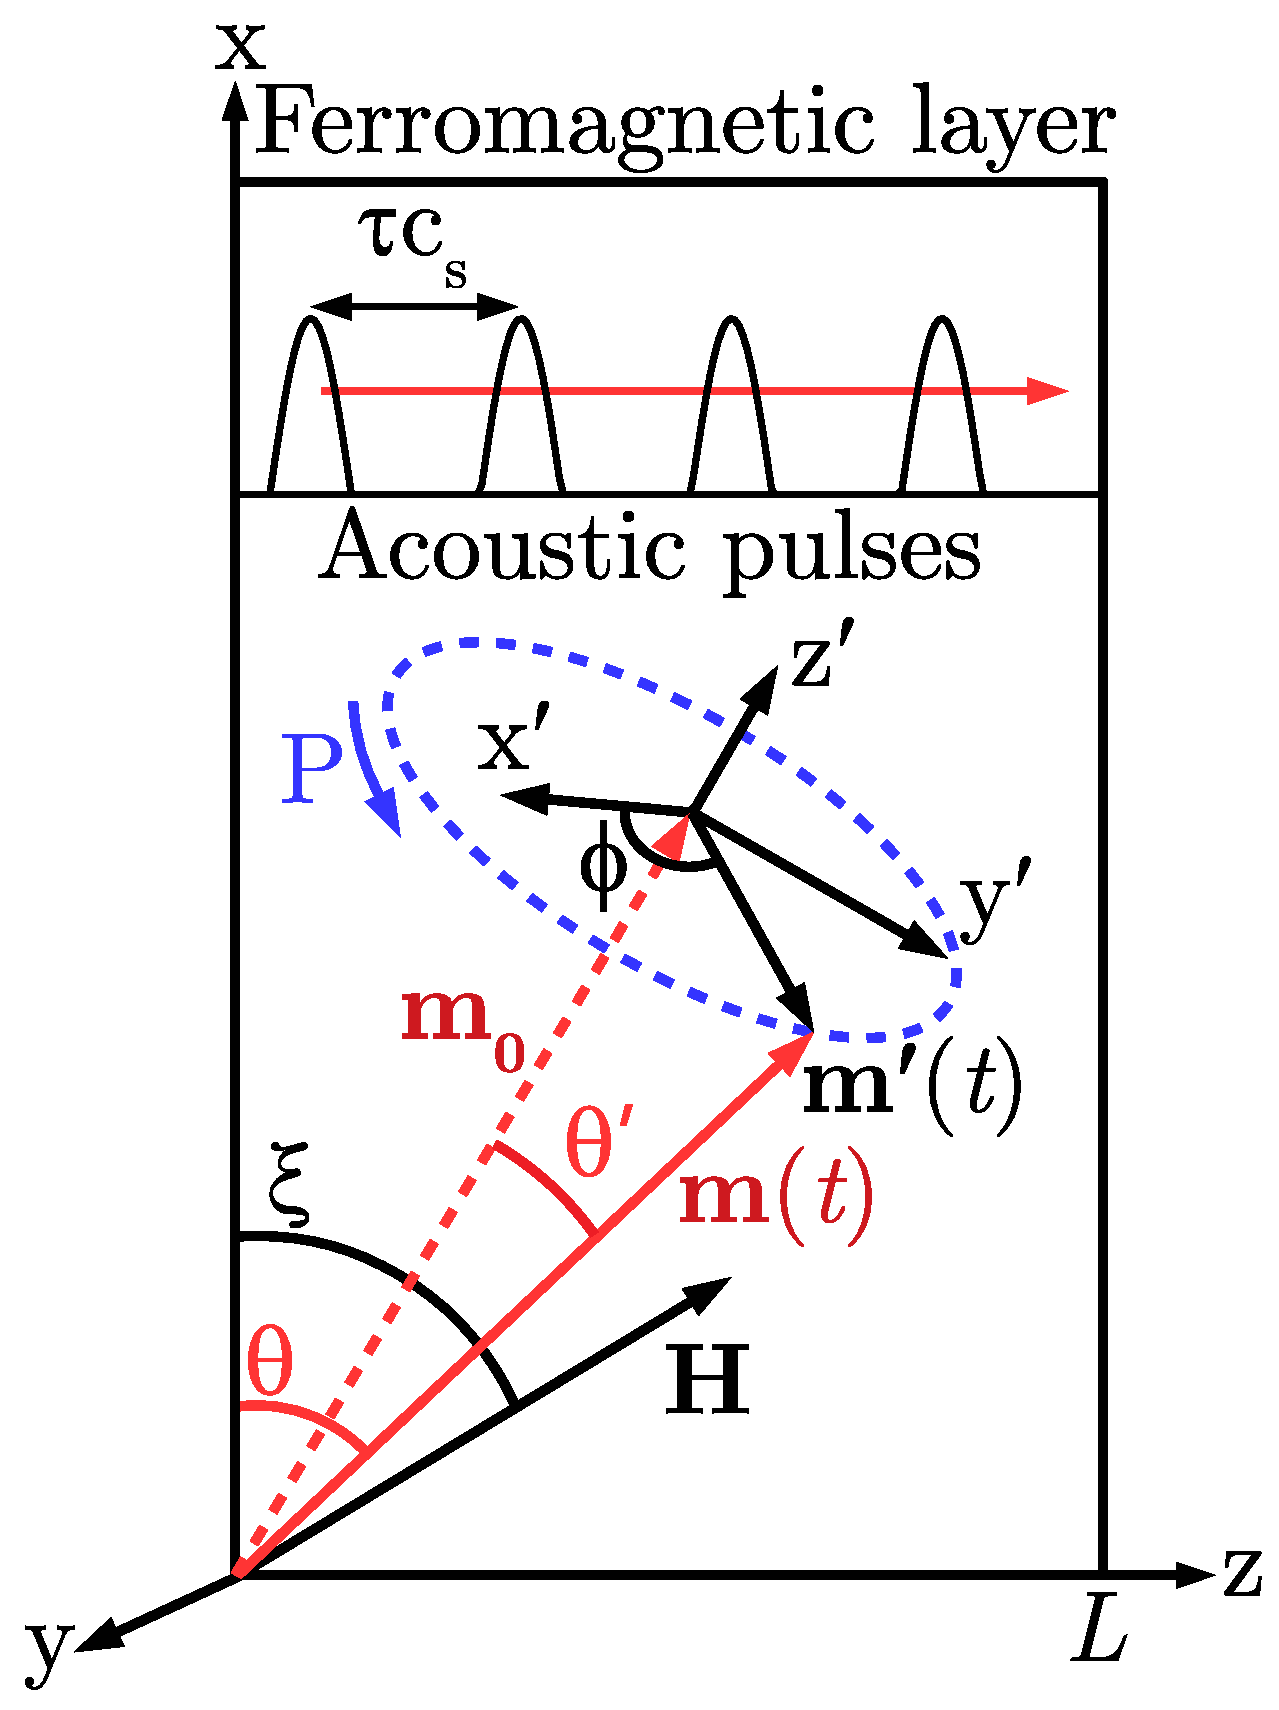
\includegraphics[width=0.4\columnwidth]{geometry_scheme.eps}}
	\hspace{0.1\columnwidth} 
    \subfloat[]{\label{fig:schemeMovement}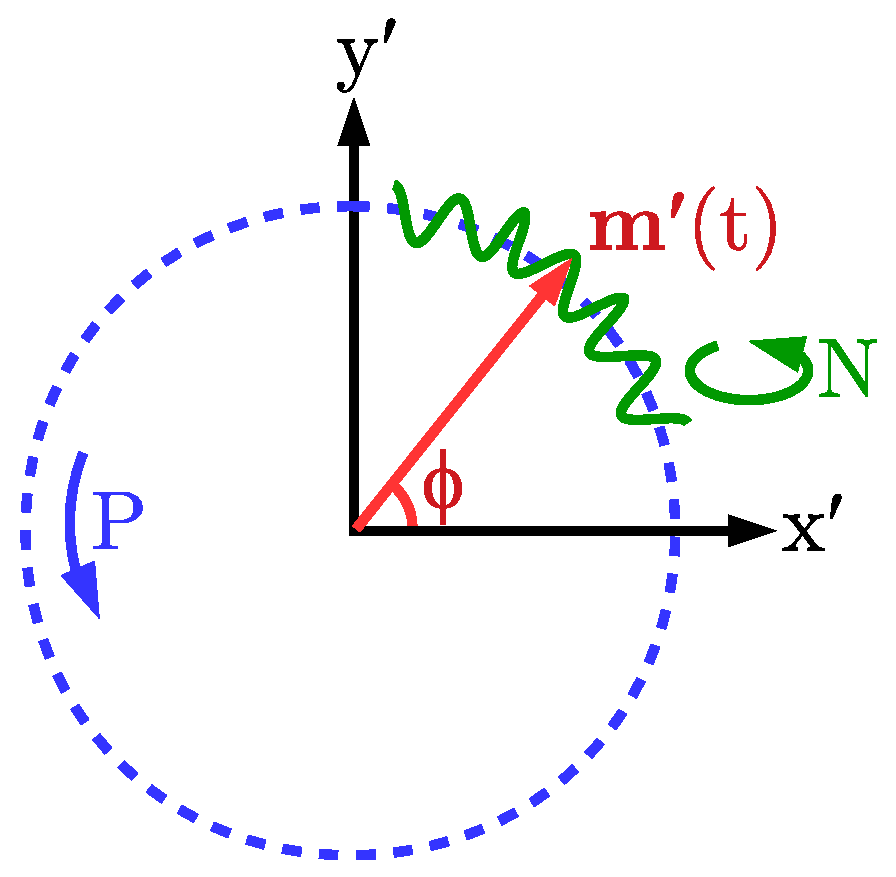
\includegraphics[width=0.4\columnwidth]{Movement.eps}}
	\caption{(Colors online) (a): Scheme of the precession P movement of the magnetization vector \textbf{m} around the equilibrium direction $\mathbf{m}_0$, induced by a train of picosecond acoustic pulses propagating with the velocity of sound $c_\mathrm{s}$ and the temporal delay $\sigma$ between the pulses. (b): Scheme of the spin movement composed by the homogeneous precession P which corresponds to the FMR and the high-frequencies non-uniform (exchange magnon) modes N.}
	\label{fig:schemes}
\end{figure}

We derived in section I of the supplementary information (SI) the Landau-Lifschitz-Gilbert (LLG) equation
\begin{equation}
	\frac{\partial \mathbf{m}}{\partial t} = - \gamma \mu_0 \mathbf{m} \left( t, z \right) \times \mathbf{H}_{\mathrm{eff}} \left( t, z \right) + \alpha \mathbf{m} \left( t, z \right) \times \frac{\partial \mathbf{m}}{\partial t}
	\label{eq:LLG}
	%\frac{\alpha}{\left| \mathbf{m}
\end{equation}
which describe the magnetization dynamic.
It includes the unit magnetization vector $\mathbf{m}\left(t,z\right)$, the gyromagnetic ratio $\gamma$, the effective magnetic field $\mathbf{H}_{\mathrm{eff}}$ and the dimensionless phenomenological Gilbert damping $\alpha$.
The magnetization vector is represented as a Fourier series in the corresponding modes 
\begin{equation}
	\mathbf{m} \left(t,z\right) = \mathbf{m}_0 + \sum_{n=0}^{N}{\mathbf{m_n}\left(t,z\right)} \cdot \cos{\frac{\pi n}{L}z}
	\label{eq:Fourier}
	%\frac{\alpha}{\left| \mathbf{m}
\end{equation}
where \textit{n} is the magnon mode number, \textit{L} is the thickness of ferromagnetic film. The constant component of the magnetization vector tilted by the theta angle with respect to the \textit{x} axis.  The second-type (free) boundary conditions for the magnetization are given
\begin{equation}
	\left.\frac{\partial \mathbf{m}}{\partial z}\right|_{z=0,L} = 0.
	\label{eq:Boundary_cond}
\end{equation}
The effective magnetic field is the variational derivative of the free energy $E$, it is defined
\begin{equation}
    \mathbf{H}_{\mathrm{eff}} = \mathbf{H}_0 + \mathbf{H}_{\mathrm{me}} + \mathbf{H}_{\mathrm{ex}},
    \label{eq:Heff}
\end{equation}
with the magnetoelastic field $\mathbf{H}_{\mathrm{me}}$ and the exchange field $\mathbf{H}_{\mathrm{ex}}$.
$\mathbf{H}_0$ is the part of the effective magnetic field which is not influence by the acoustic strain
\begin{equation}
    \mathbf{H}_0  \mathbf{H}_{\mathrm{de}} + \mathbf{H}_{\mathrm{z}},
\end{equation}
with $\mathbf{H}_{\mathrm{de}}$ the demagnetization field and $\mathbf{H}_{\mathrm{z}}$ the external magnetic field.
As derived in section II of the SI, we investigate the strain dependence of two field: the exchange field and the magnetoelastic field.
While the variation of the magnetoelastic field due to the acoustic strain can generate several exchange magnon modes and propagate through the sample when the magnetization vector is equal to $\mathbf{m}_0$,
the exchange field terms only occur in the parametric terms of Eq. \eqref{eq:LLG}.
The parameters used in our simulation are presented in table ... in the SI.
%This situation can be realized in an optical pump-probe experiment using a train of laser pump pulses. 
%Absorption of each pump pulse leads to the excitation of an acoustic pulse. 
%The LLG equation can be written for each magnetization component. 
%We calculate the analytic dispersion relation for the magnon.
%We study the excitation of exchange magnons in nickel thin film. 
%By varying the magnitude of the magnetic field it is possible to tune the magnon dispersion curve and select which magnon mode we want to excite. 
%However the spinwaves could be highly damped.
%Another limiting factor maybe the duration of the acoustic pulses. It should be investigate.

Before considering a series of acoustic pulse, it is important to investigate the precession angle response as a function of the strain amplitude in order to find the range at which we have a linear response.
We calculate the precession angle due to the propagation of an acoustic strain for different amplitude.
We set the external magnetic field's magnitude to $6.54\ \mathrm{T}$, the other parameters are shown in Table 1 of Section 3 in the SI.
Table \ref{tab:StrainAmplitudeVSPrecessioAngle} shows the precession angle ($\theta'$) variation as a function of the strain amplitude ($\left| \epsilon_{zz} \right|$).
We consider the excitation induced by only one acoustic pulses while the external magnetic field's magnitude is set to $6.45\ T$.
It appears that for a strain's amplitude smaller than $1\ \%$, the precession angle evolve linearly.
We fix the strain amplitude to $0.5\ \%$.
\begin{table}[b]
    \centering
    %\begin{tabular}{p{4cm} p{4cm} p{4cm} p{4cm}}
    \begin{tabular}{C{4cm} C{4cm} C{4cm} C{4cm}}
        \hline
        \hline
        %Strain amplitude & Average precession angle (degree) & Standard deviation (degree)  & Maximal value of the precession angle \\
        $\left| \epsilon_{zz} \right|$ (\%) & $<\theta'>$ (degree) & $\sigma$ & $\theta'_{\mathrm{max}}$ \\
        \hline
        $0.1$ & $1.35 \times 10^{-3}$ & $1.19 \times 10^{-3}$ & $5.83 \times 10^{-3}$ \\
        $0.2$ & $5.42 \times 10^{-3}$ & $4.79 \times 10^{-3}$ & $2.35 \times 10^{-2}$ \\
        $0.3$ & $1.22 \times 10^{-2}$ & $1.08 \times 10^{-2}$ & $5.35 \times 10^{-2}$ \\
        $0.4$ & $2.17 \times 10^{-2}$ & $1.92 \times 10^{-2}$ & $9.6 \times 10^{-2}$ \\
        $0.5$ & $3.38 \times 10^{-2}$ & $3 \times 10^{-2}$ & $1.51 \times 10^{-1}$ \\
        $0.75$ & $7.62 \times 10^{-2}$ & $6.76 \times 10^{-2}$ & $3.5 \times 10^{-1}$ \\
        $1$ & $1.36 \times 10^{-1}$ & $1.21 \times 10^{-1}$ & $6.37 \times 10^{-1}$ \\
        $1.5$ & $3.05 \times 10^{-1}$ & $2.73 \times 10^{-1}$ & $1.51$ \\
        $2$ & $5.43 \times 10^{-1}$ & $4.92 \times 10^{-1}$ & $2.84$ \\
        $2.5$ & $8.49 \times 10^{-1}$ & $7.8 \times 10^{-1}$ & $4.7$ \\
        $3$ & $1.22$ & $1.14$ & $7.16$ \\
        \hline
        \hline
    \end{tabular}
    \caption{Influence of the strain amplitude ($\left| \epsilon_{zz} \right|$) on the precession angle ($\theta'$). We report also the standard deviation ($\sigma$) and the maximal value reach by the precession angle ($\theta'_{\mathrm{max}}$).}
    \label{tab:StrainAmplitudeVSPrecessioAngle}
\end{table}
\begin{figure}
    \centering
    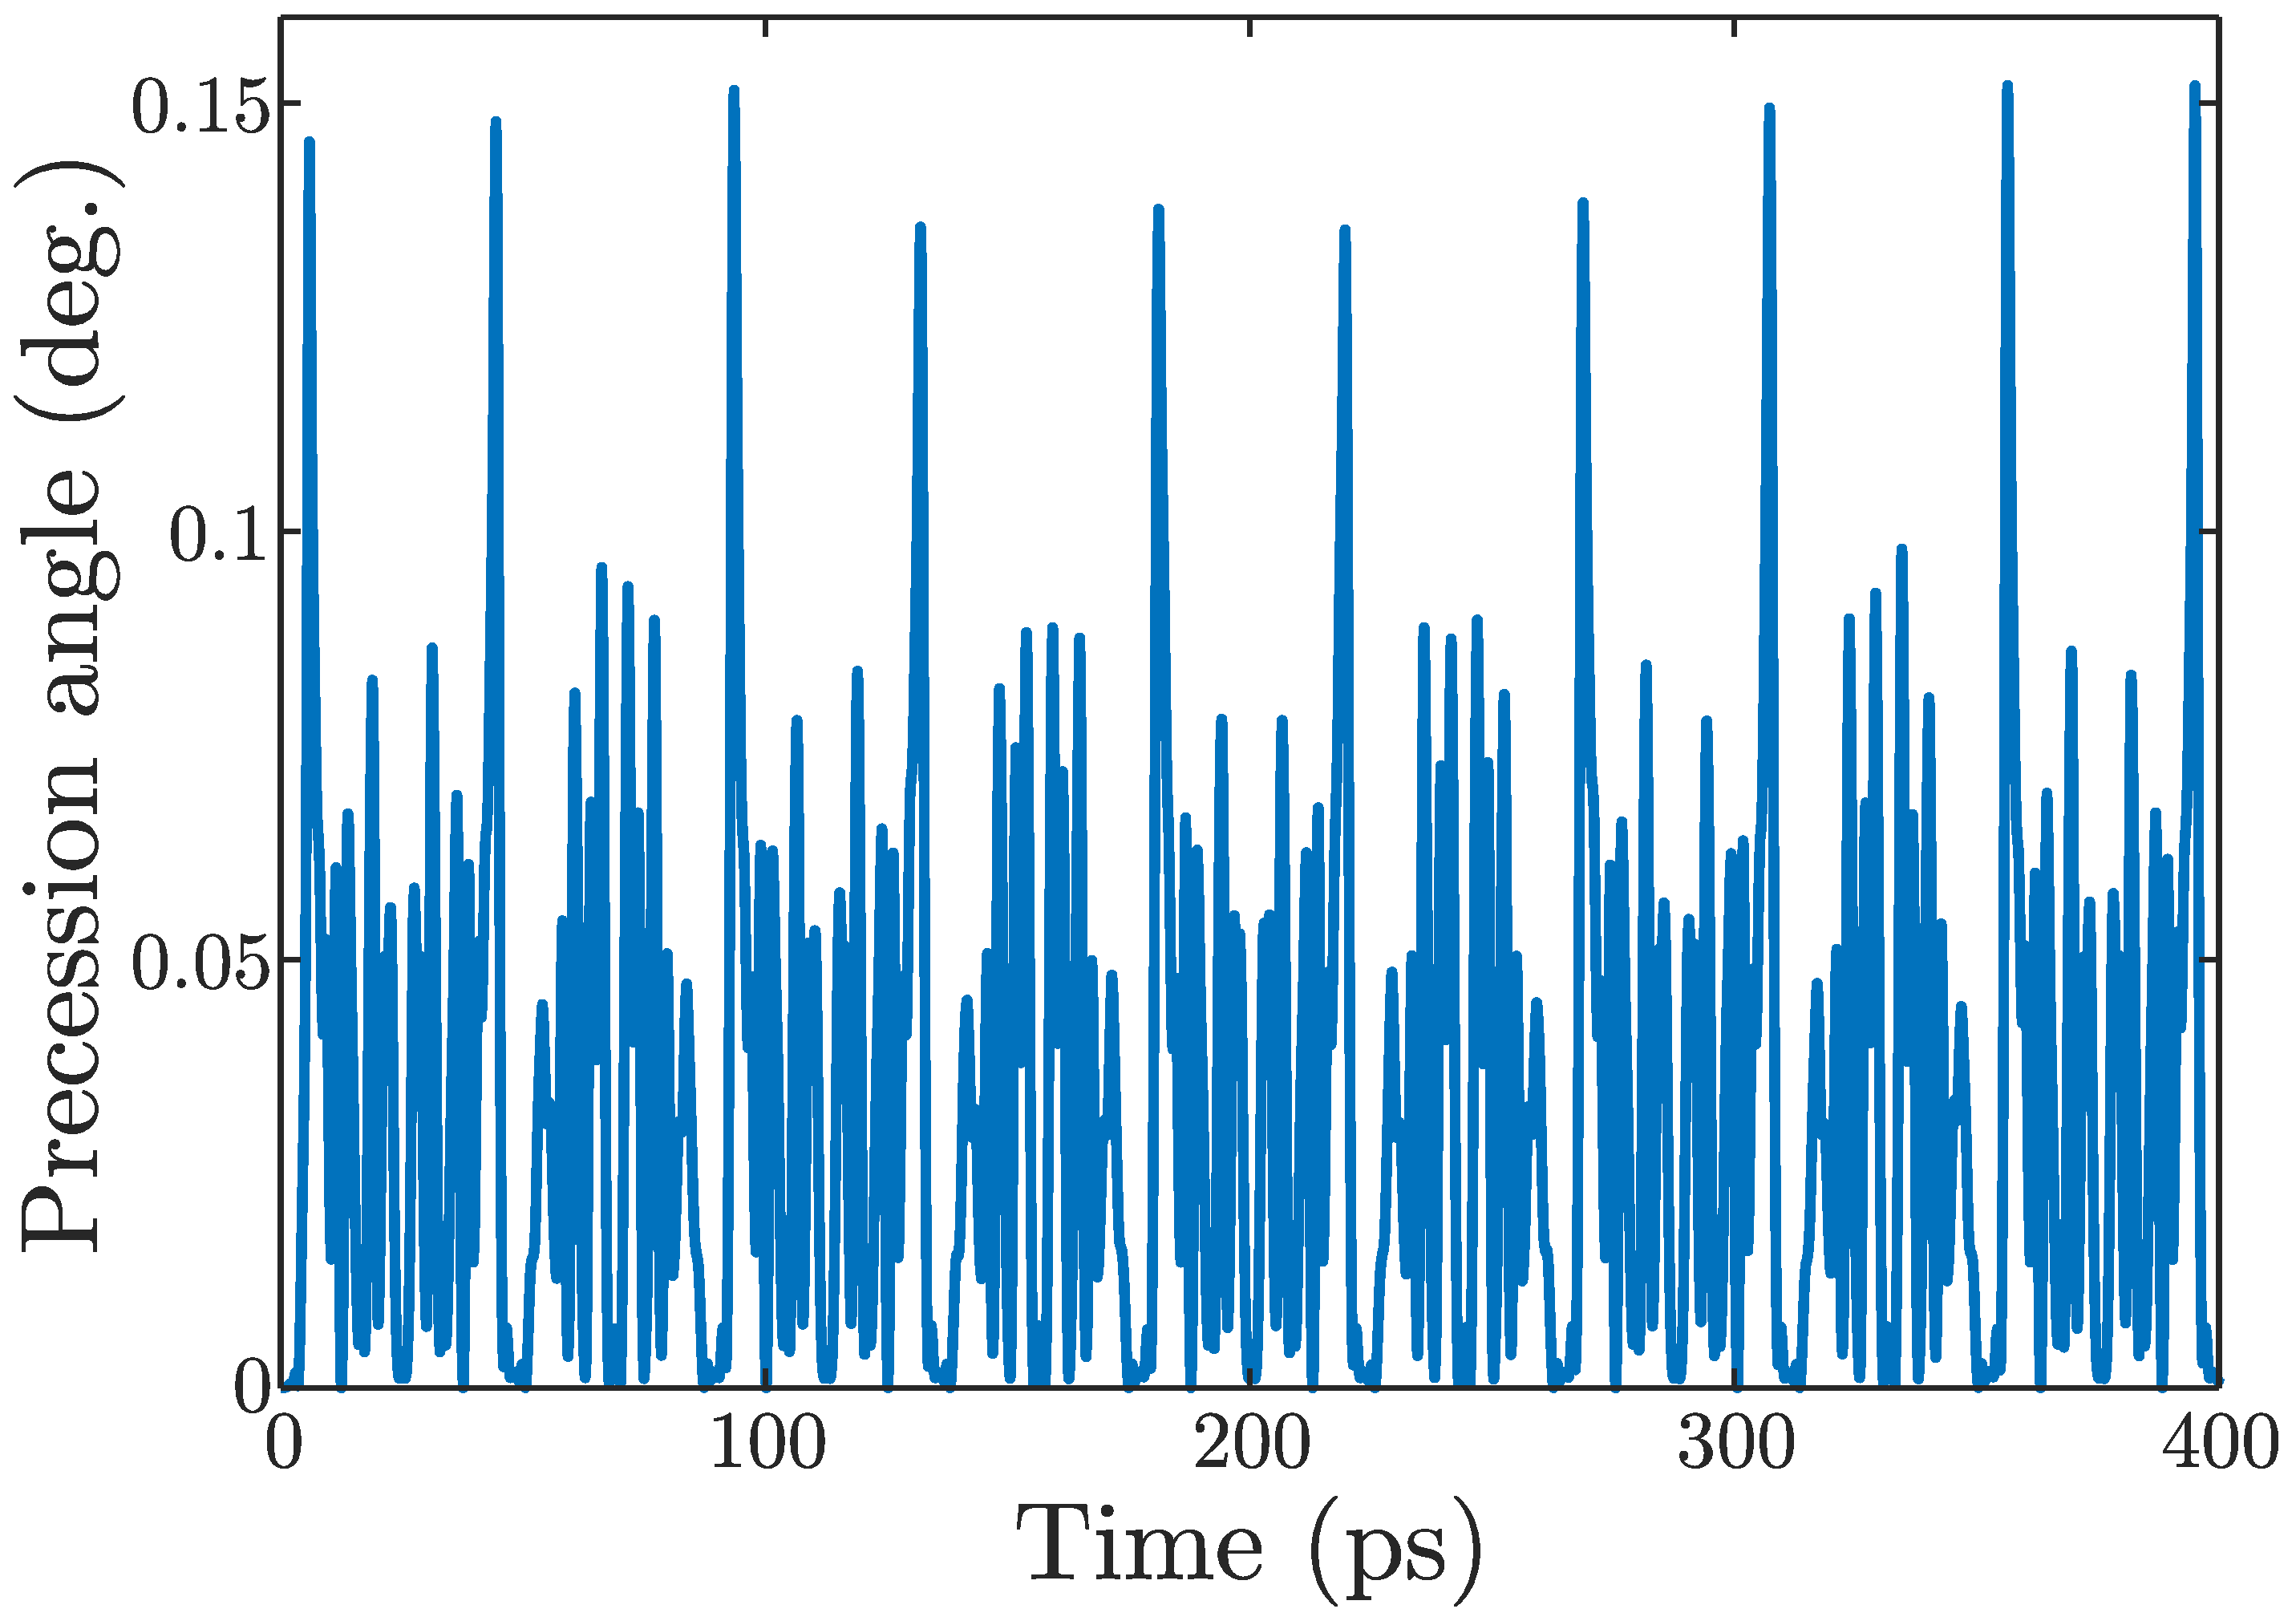
\includegraphics[width = 0.95\columnwidth]{Figures/precessionAngle05.eps}
    \caption{Precession angle (deg.) as a function of the time (ps) due to the propagation of one acoustic pulse with a $0.5\%$ strain amplitude.}
    \label{fig:precessionAngle05}
\end{figure}

The behavior of the magnetization vector can be estimated through the characteristics of the dispersion curves of acoustic and spinwaves branches. By playing with the magnetic field we can tune the spinwave dispersion curve. So we can choose the magnitude of the field in such a way that there is none, only one or two intersection points between acoustic and spinwave dispersion curves. For the case of one intersection point phase velocity of magnons and acoustic pulses will be equal. In this case the most suitable frequency is close to 500 GHz. It corresponds to a delay of 2 ps between the acoustic pulses.
	
\begin{figure}[ht]
	\centering
	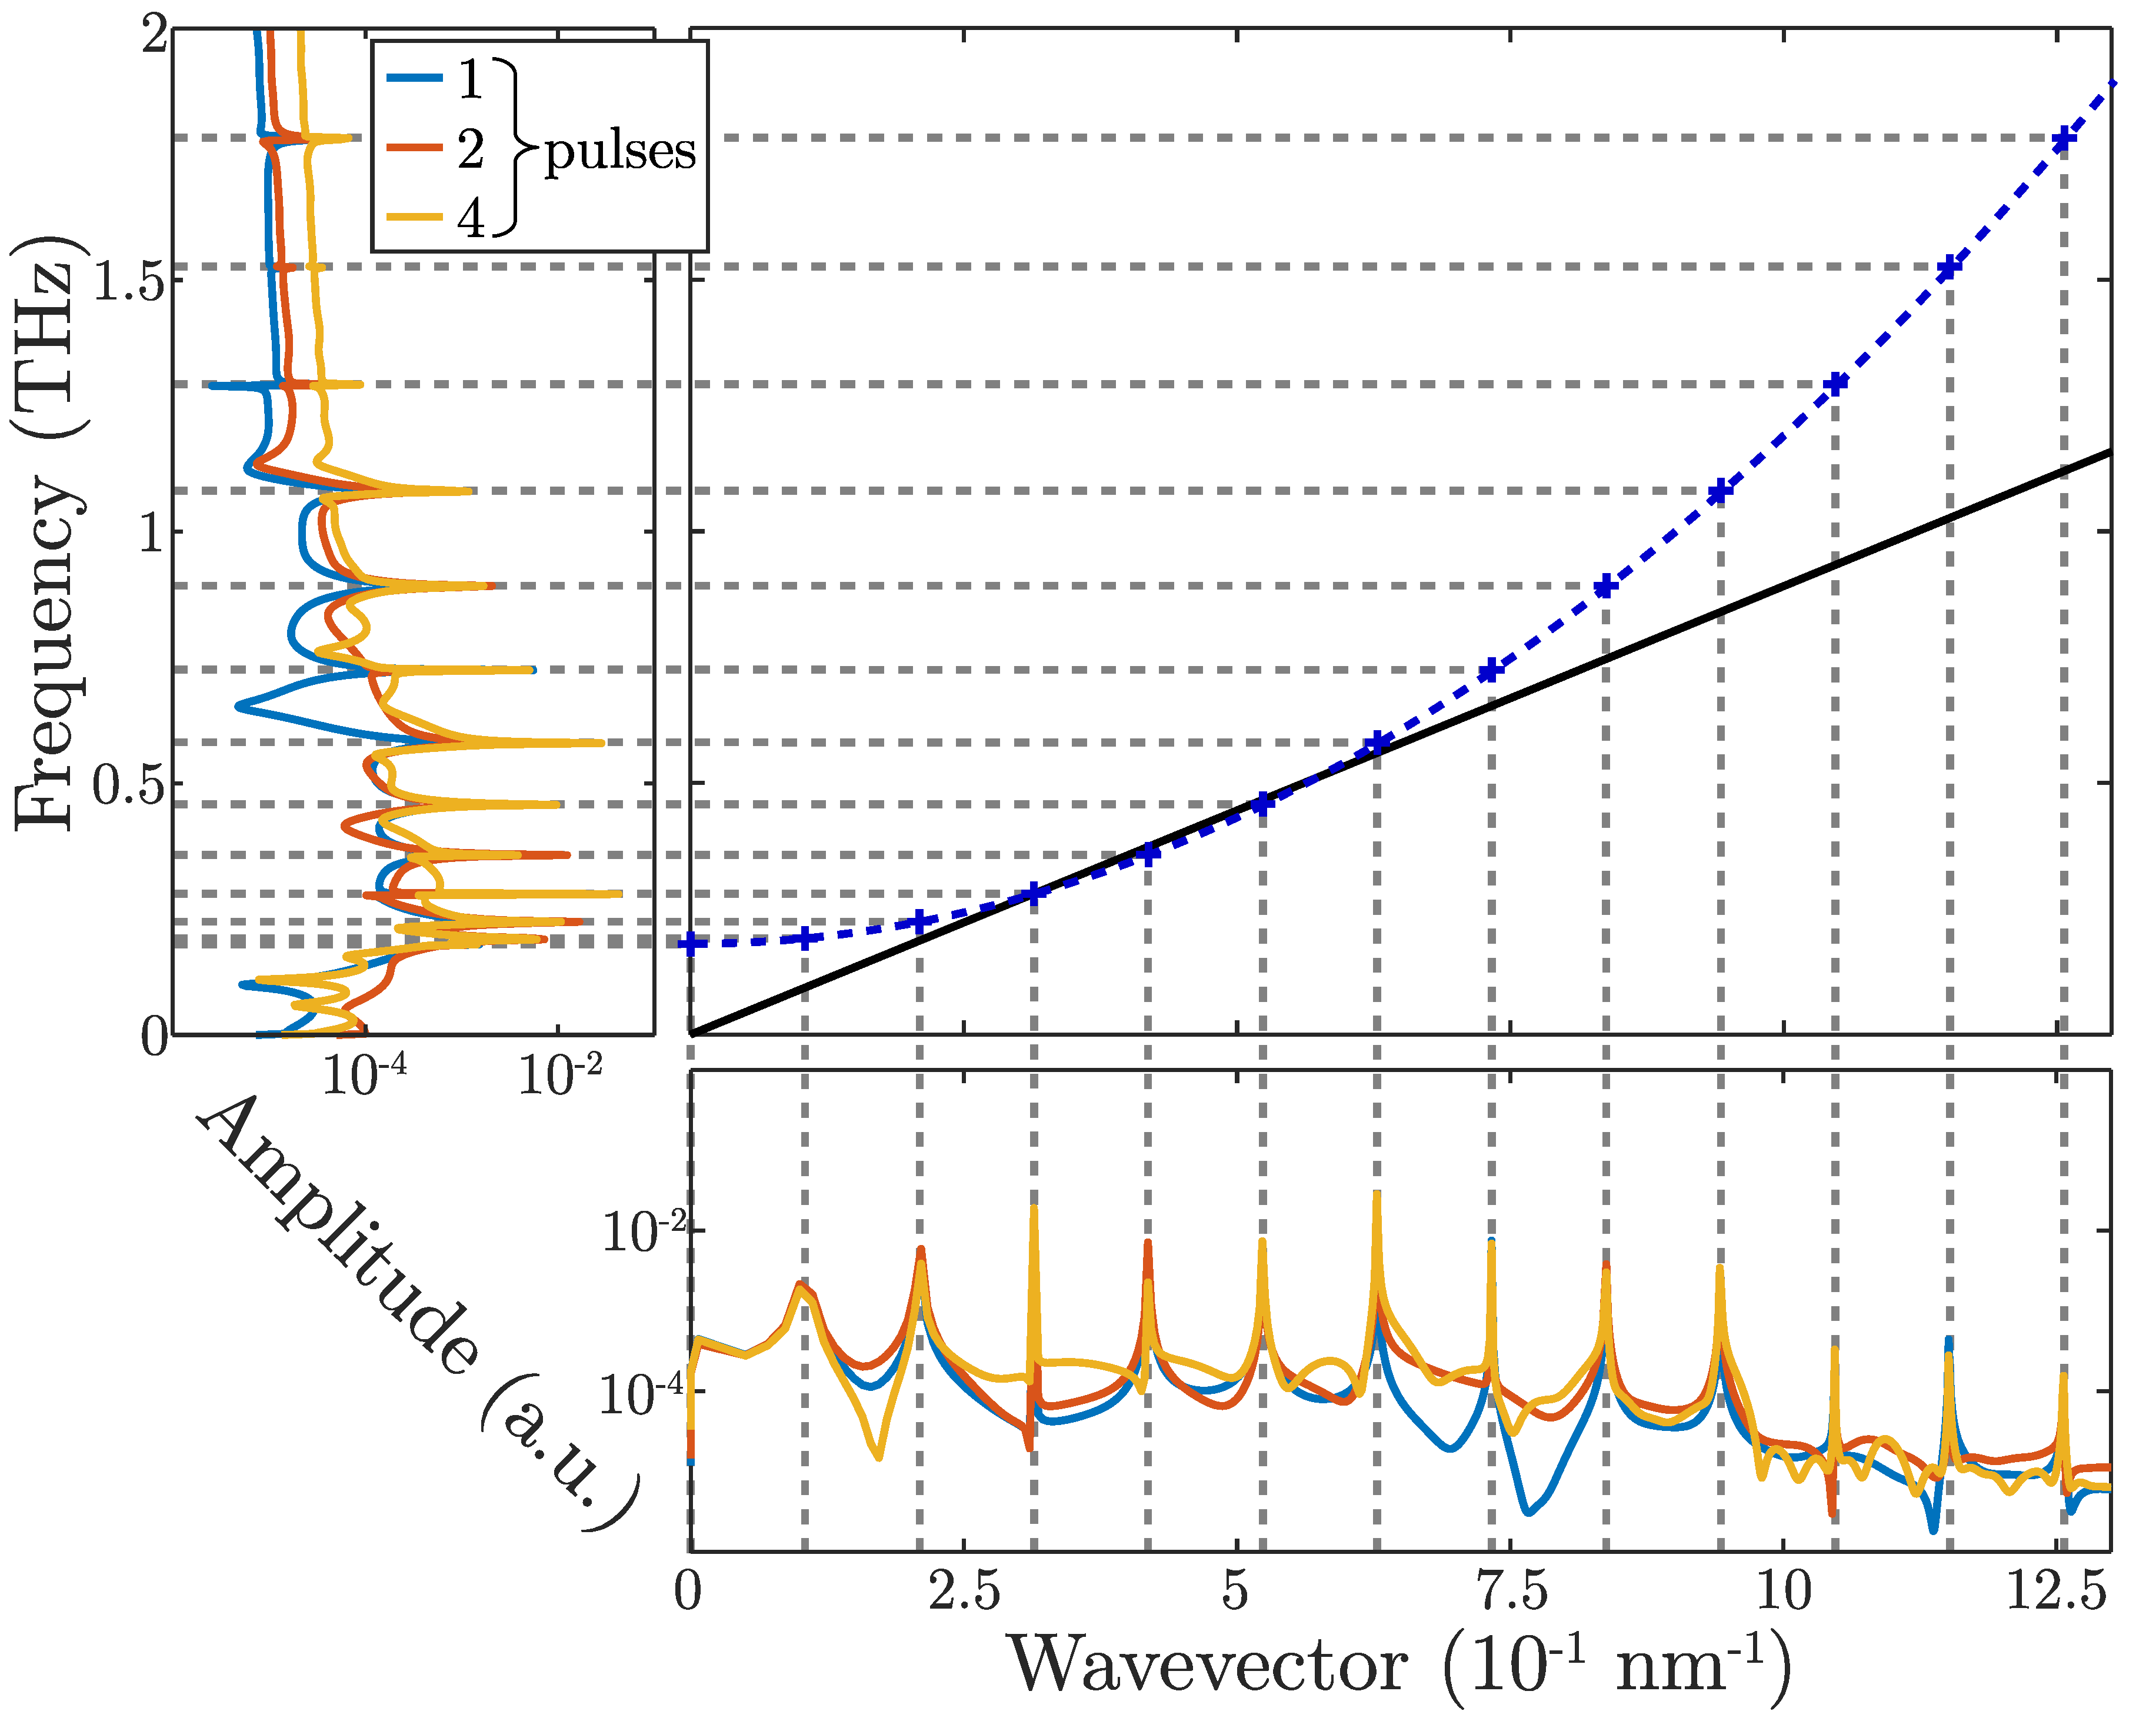
\includegraphics[width=0.95\columnwidth]{Figures/dispersionRelation-H6.5T-Ni30nm-3.57_2ps.eps}
	\caption{Acoustic dispersion relation curve (black line) and magnon dispersion relation curve for $H = 6.5\ \mathrm{T}$ (blue dashed line). The left figure corresponds to the spectrum of the magnetization as a function of the frequency (THz) while the bottom figure corresponds to same spectrum but as a function of the wavevector ($10^{-1}\, \mathrm{nm}^{-1}$). The blue, red and yellow curves corresponds to the magnetization resulting from an excitation due to a serie of, respictively, one, two and four acoustic pulses. The repetition frequencies of the acoustic pulses is 280.1 GHz.}
	\label{fig:dispersionRelationHNi}
\end{figure}
	
Acoustic and magnon dispersion relation curves for a magnitude of the DC magnetic field equals to 6.5 T and angle $\xi = 45^{\circ}$  are shown in Fig.~\ref{fig:dispersionRelationHNi}. Two intersection points on the dispersion curves in Fig. 2 can be seen. Parameters of the acoustic pulses that correspond to the left intersection point were taken. The duration of a single acoustic pulse is 1 ps and time between acoustic pulses equals to 3.57 ps which corresponds to the frequency between pulses equals to 280.1 GHz for the case of several pulses in the series.
	
The spectrum of the magnetization dynamics in nickel thin film excited by a series of picosecond acoustic pulses with the parameters described above shown in the left part of Fig.~\ref{fig:dispersionRelationHNi}. The largest contribution to the spectrum was made by the frequency corresponding to the frequency of the intersection point of the acoustic and spinwave dispersion branches regardless of the number of pulses. Subharmonics and harmonics of a higher order are also excited. The frequency difference between adjacent peaks increases linearly with increasing mode number (Fig.~\ref{fig:dF_regularity}).
	
\begin{figure}[ht]
	\centering
	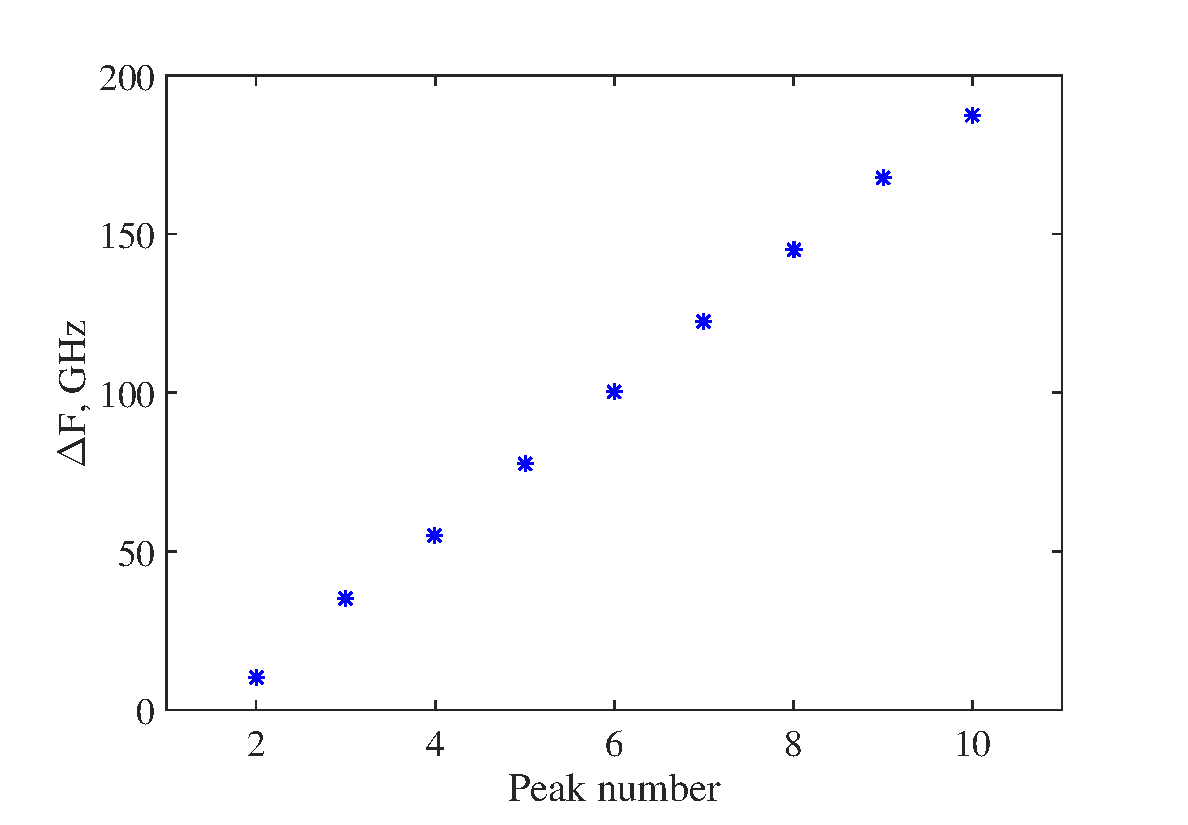
\includegraphics[width=0.95\columnwidth]{dF_regularity.eps}
	\caption{The dependence of frequency difference between adjacent peaks from peak number.}
	\label{fig:dF_regularity}
\end{figure}
	
The amplitude of the excited oscillations can be amplified by increasing the number of acoustic pulses. Changing the number of acoustic pulses and time between them we can strengthen certain harmonics and jam the others. This is significantly determined by the spectrum of the initial acoustic signal and the frequencies present in it.
	
Fig.~\ref{fig:spectrumUniBip} shows the oscillation spectra for series of four acoustic pulses of unipolar and bipolar forms. Excitation occurs at the same frequencies as can be seen from the spectra of the excited oscilations. A unipolar pulses gives a greater contribution to the relatively lower frequencies and bipolar pulses to higher ones. It is determined by the spectrum of the initial acoustic signal. For a unipolar pulses the peak of the spectral dependence is shifted to low frequencies and for the bipolar pulses to high frequencies. This is due to the fact that for the acoustic bipolar pulses of 1 ps duration the maximum in spectrum is close to 1 THz. But since the spectra are similar it is possible to change the amplitude of acoustic pulses to achieve the same effects for certain modes or frequencies as if a transition from a unipolar form of acoustic pulses to a bipolar one were used.
	
\begin{figure}[ht]
	\centering
	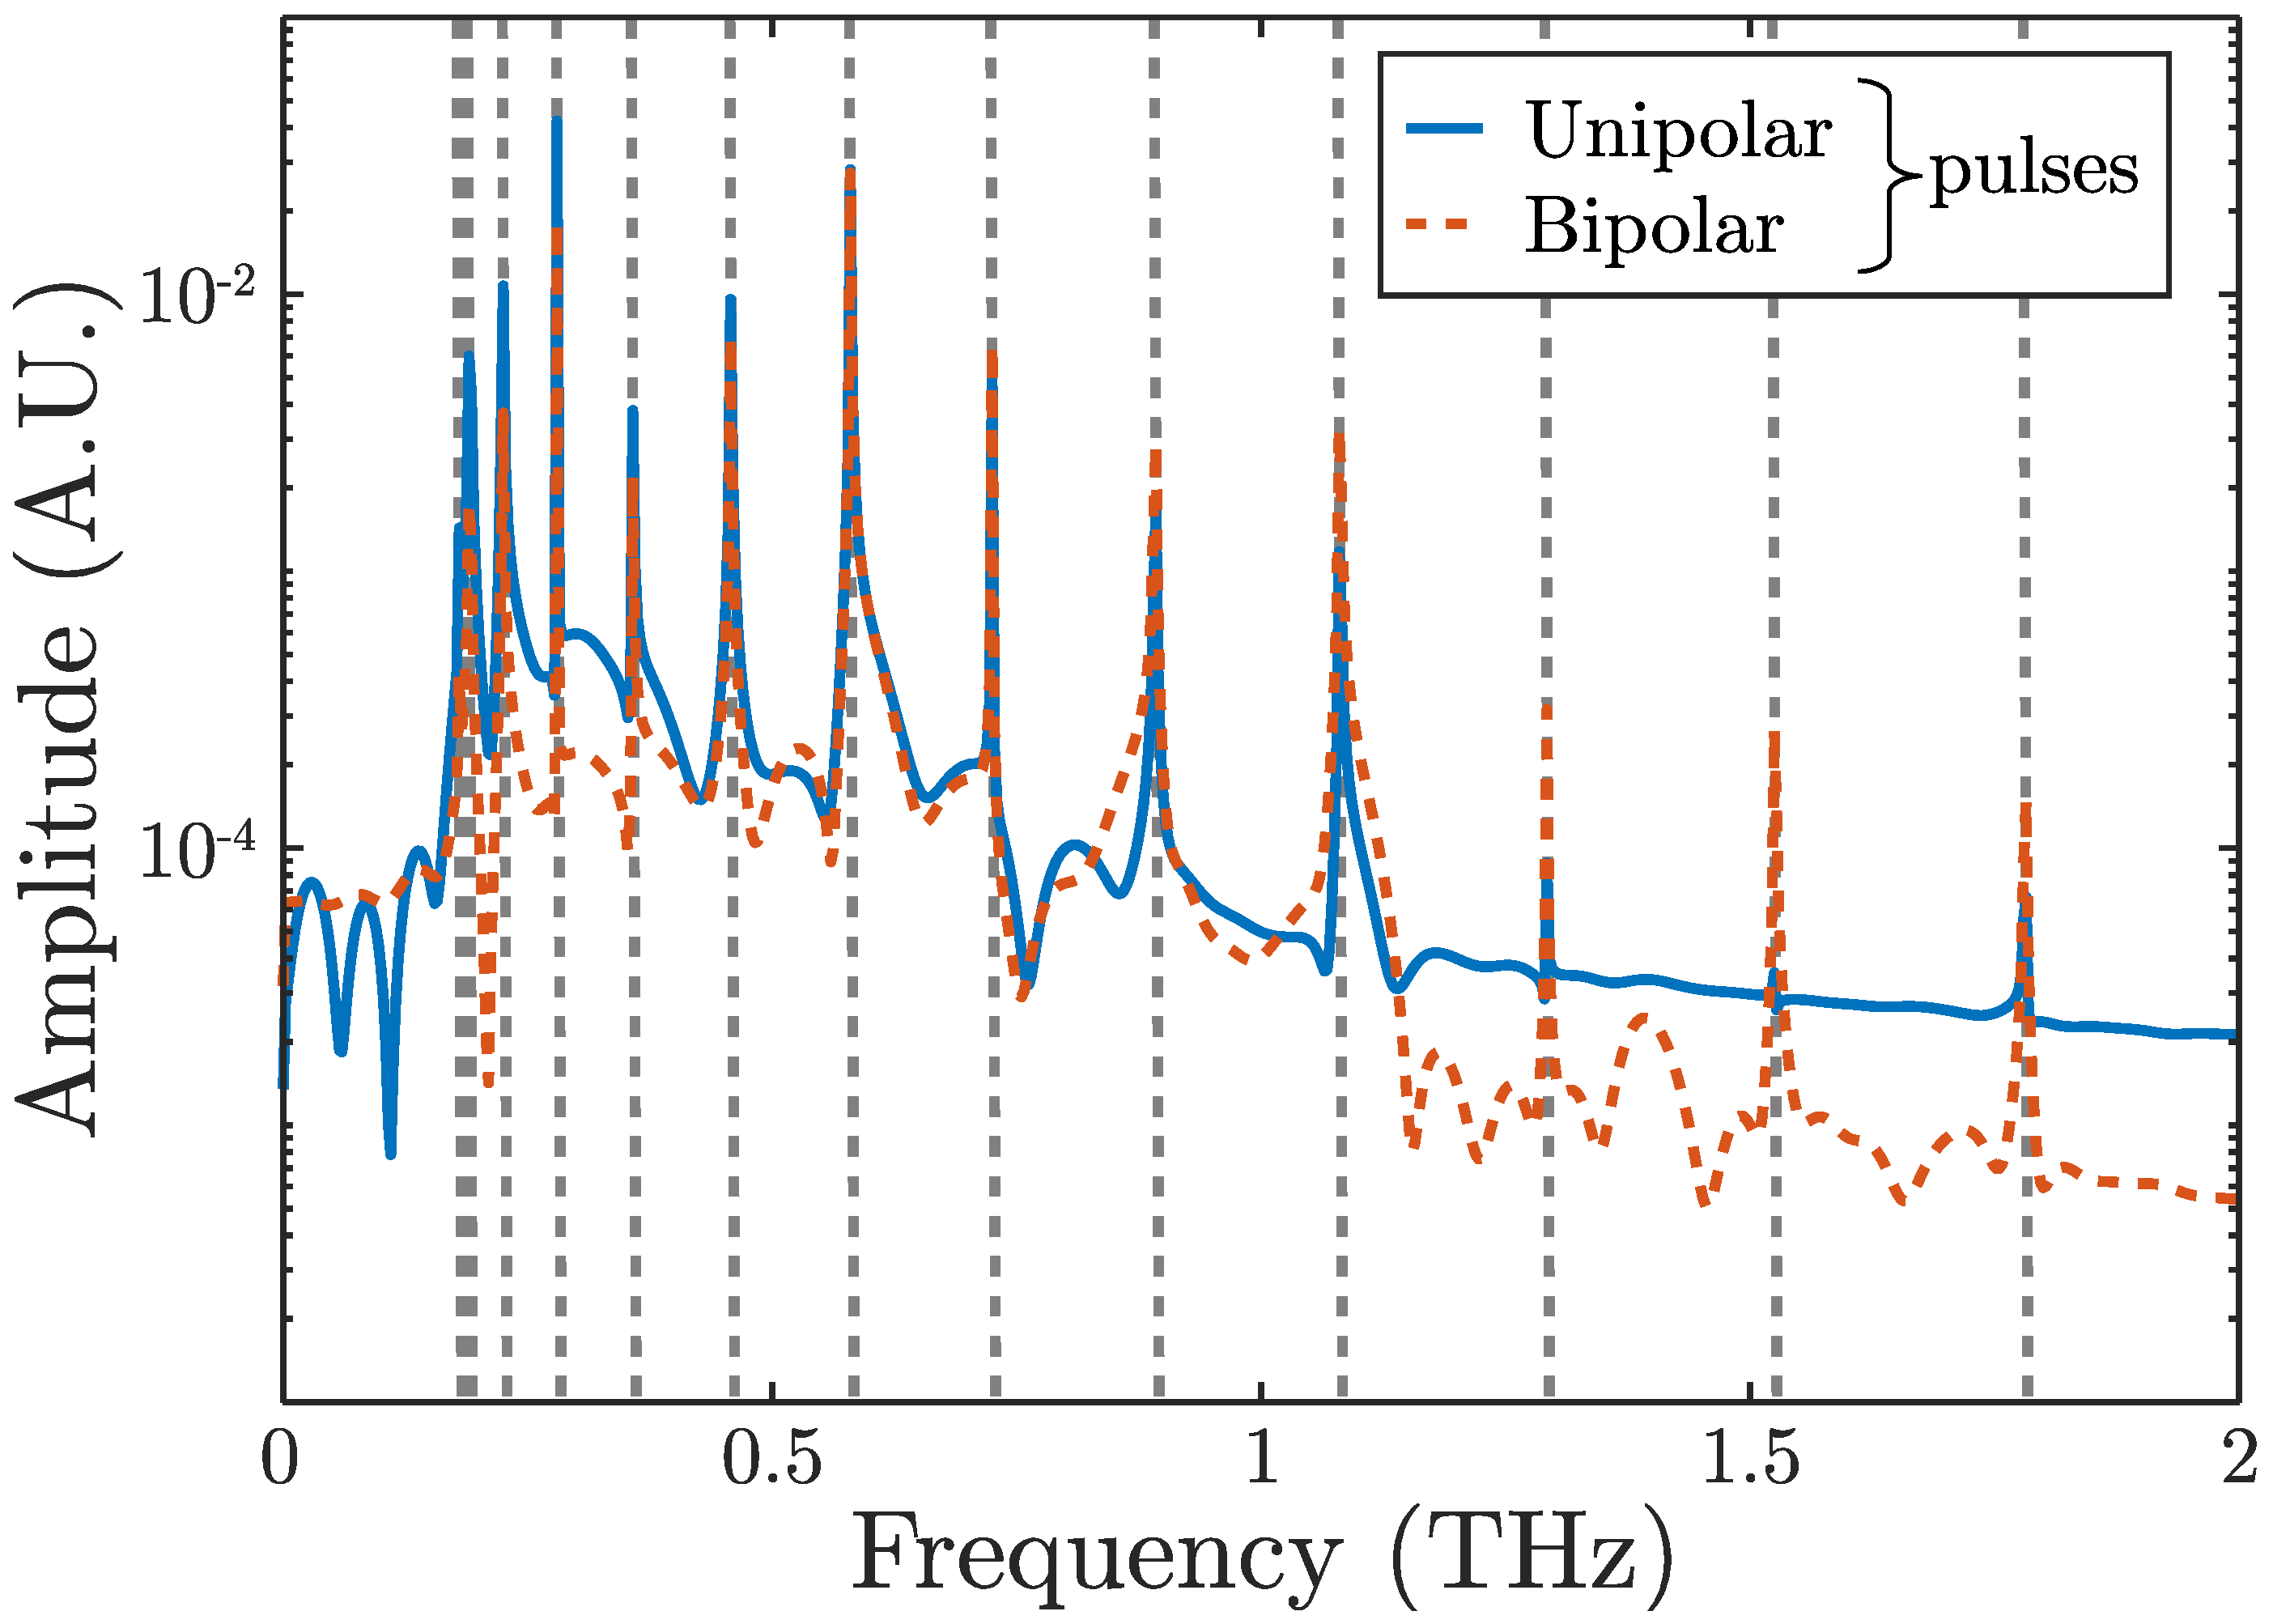
\includegraphics[width=0.95\columnwidth]{spectrumLogNorm-Ni_30nm-6_5T-uni_bip-3_57ps-withMode.eps}
	\caption{(Colors online) Unipolar and bipolar.}
	\label{fig:spectrumUniBip}
\end{figure}
	
\begin{figure}[ht]
	\centering
	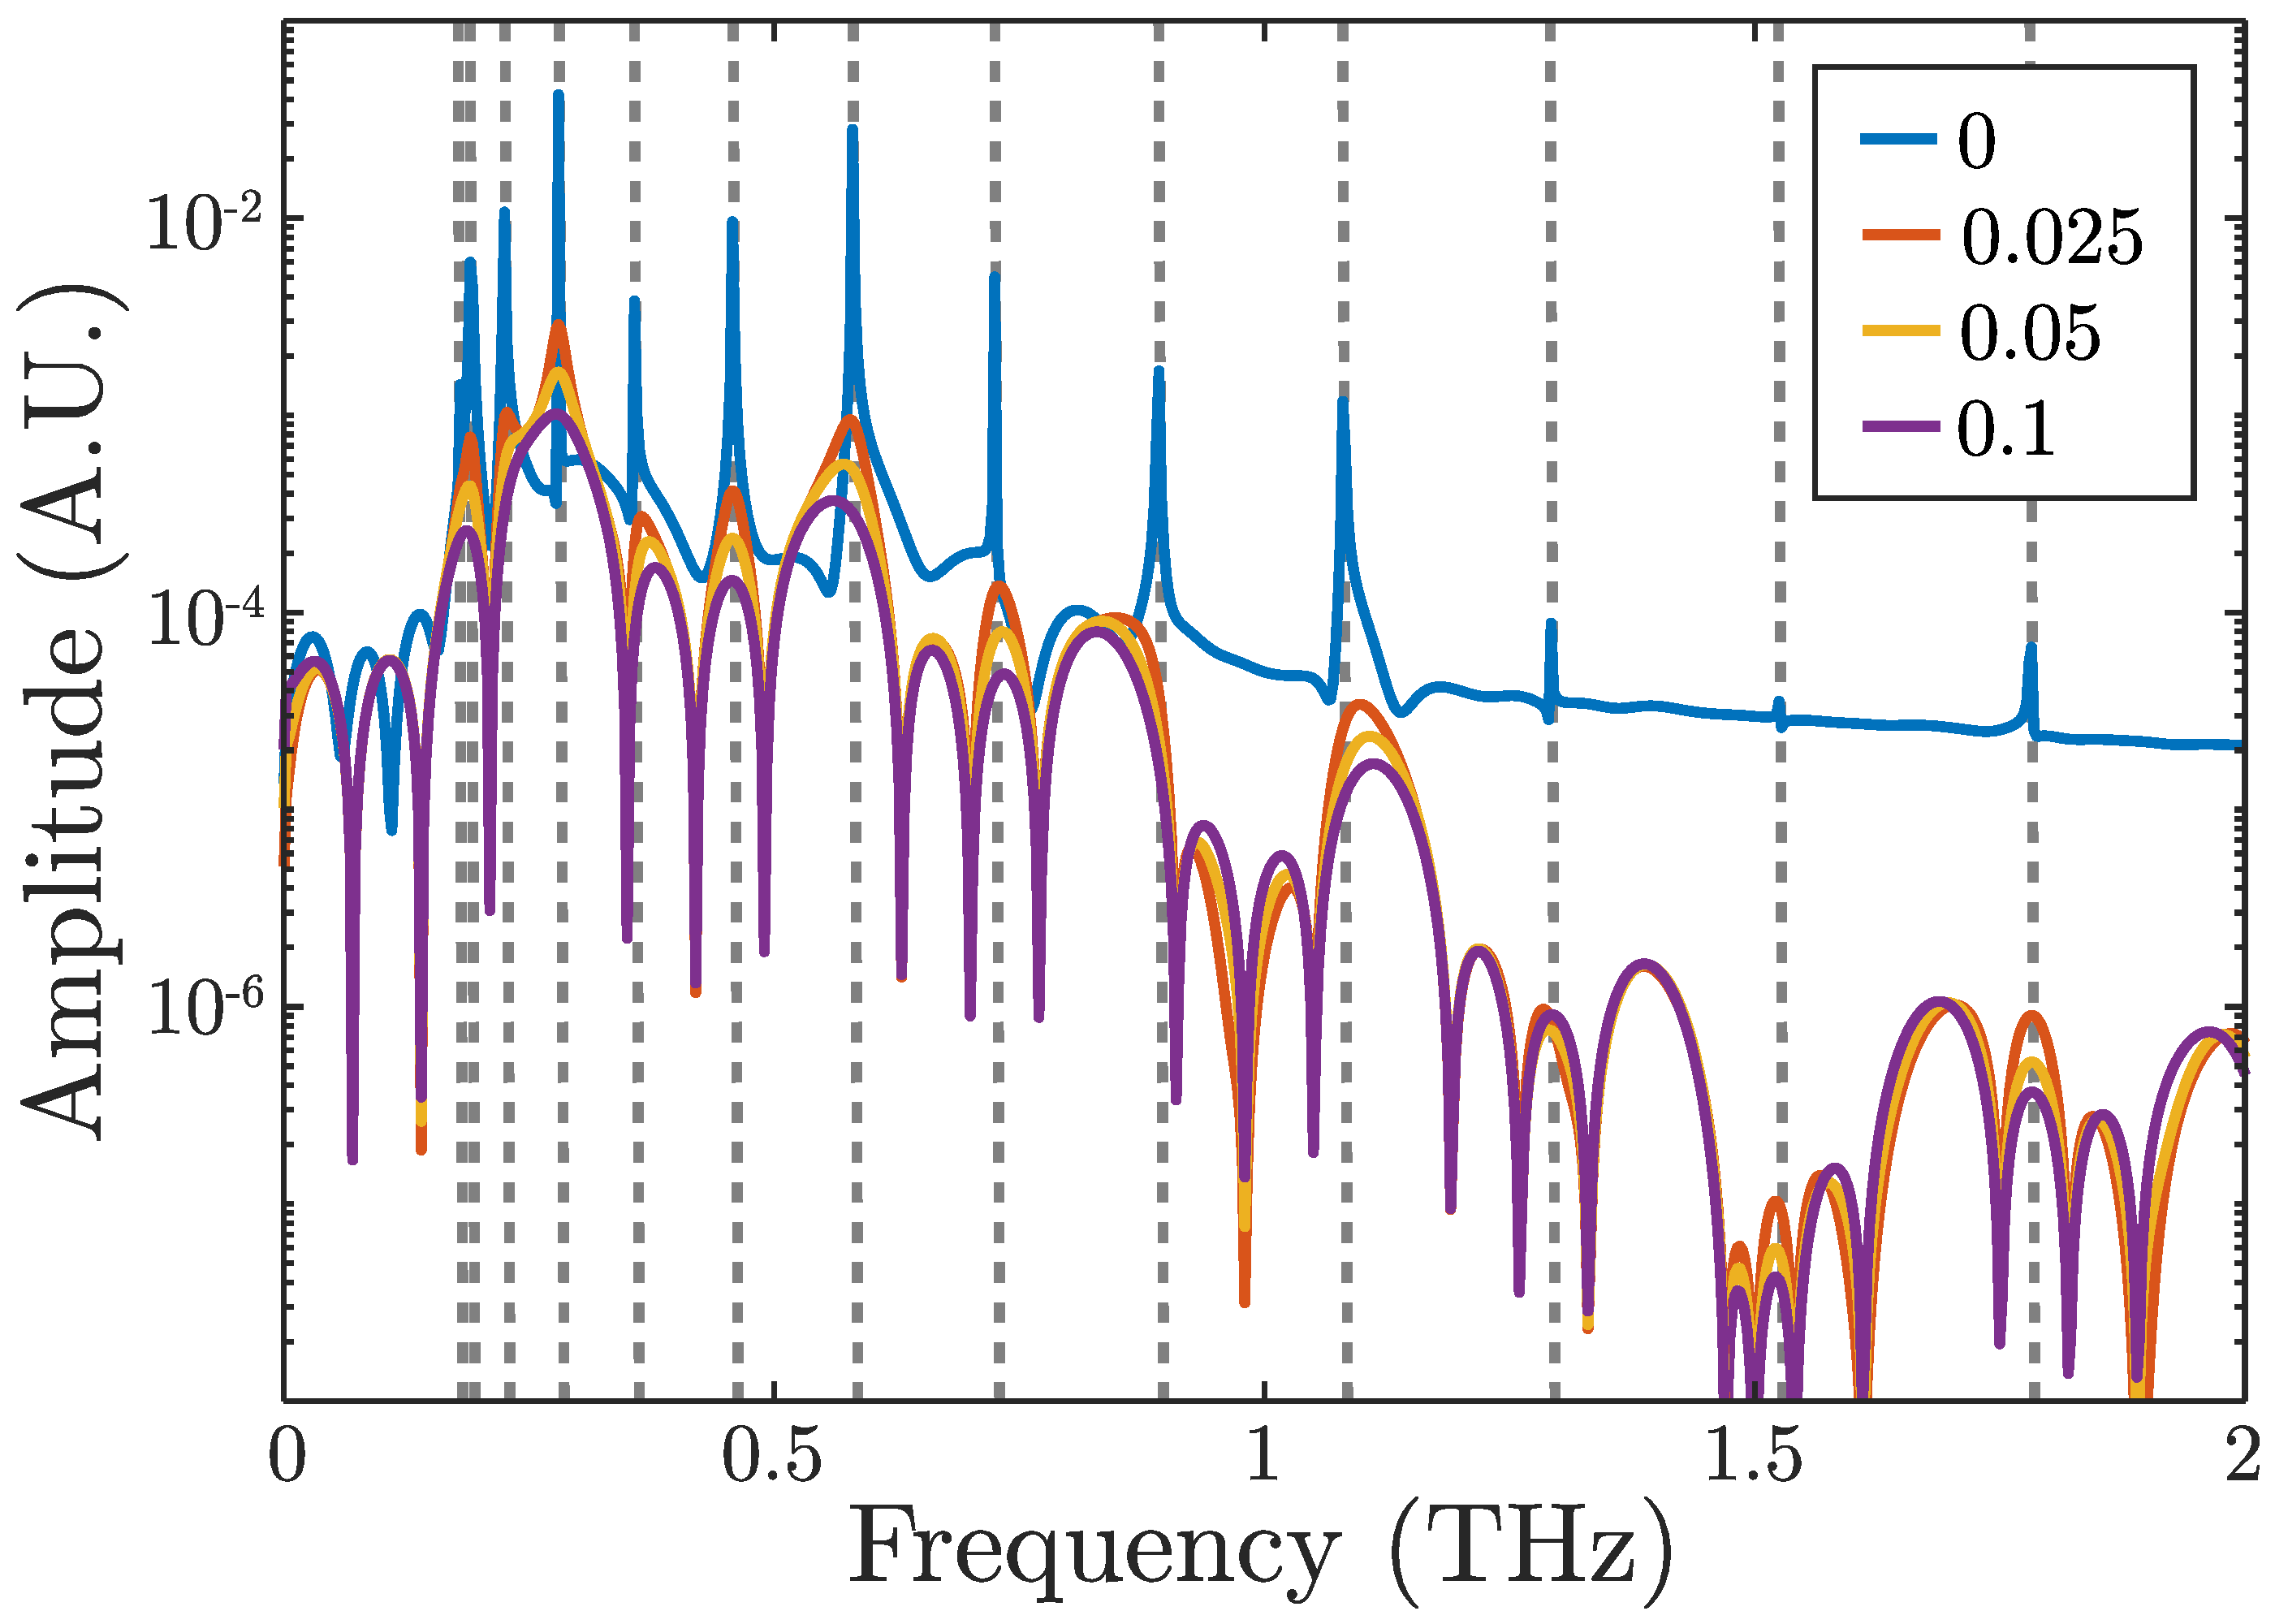
\includegraphics[width=0.95\columnwidth]{spectrumDampingNormLog-Ni_30nm-6_5T-uni-3_57ps-withMode.eps}
	\caption{(Colors online) Damping.}
	\label{fig:spectrumUniDamping}
\end{figure}
	
The oscillation spectra for series of four unipolar acoustic pulses for different damping parameters $\alpha$ shown on Fig.~\ref{fig:spectrumUniDamping}. The presence of damping significantly affects the shape of the spectral dependence. The highfrequency parts of the excited oscillations decay most rapidly. The oscillation spectrum begins to repeat the spectrum of the initial acoustic signal at large damping parameters.
	
%We studied the excitation of exchange magnons in nickel thin film. By varying the magnitude of the magnetic field It is possible to drive the magnetization with acoustic pulses by playing on their shapes, their number and the delay between them.The spinwaves could be highly damped, making them more difficult to detect.

In conclusion, we reported a study of exchange magnons in nickel thin films excited by a series of picosecond acoustic pulses.
Our model described the generation and the propagation of a spinwave packet due to the propagation of acoustic pulses through the nickel film.
The magnetization dynamics movement can be decomposed in a precession and a nutation movement in the precession's plane.
We demonstrate the we excited high order magnons and it is possible to enhance this excitation by playing on the delay between the successive acoustic pulses in order to match the phase velocity condition.
	
\bigskip
	
Funding through Nouvelle \'{e}quipe, nouvelle th\'{e}matique "Ultrafast acoustics in hybrid magnetic nanostructures", Strat\'{e}gie internationale NNN-Telecom and the Acoustic HUB de la R\'{e}gion Pays de La Loire, Alexander von Humboldt Stiftung, the European Research Council (FP7/2007-2013) / ERC grant agreement no. 306277 and PRC CNRS-RFBR "Acousto-magneto-plasmonics" (grant number 1757 150001) is greatfully acknowledged.
	
\bibliographystyle{apsrev4-1} % Tell bibtex which bibliography style to use
\bibliography{bib_ExchangeMagnons}
	
\end{document}